\documentclass{article}
\usepackage[utf8]{inputenc}
\usepackage{tikz}
\usetikzlibrary{shapes,arrows}

\title{Research Workflow}
\author{Jawad Khan}
\date{December 10 2017}

% Define block styles
\tikzstyle{topic} = [rectangle, minimum width=3cm, minimum height=1cm, text centered, draw=black, fill=red!30]
\tikzstyle{decision} = [rectangle, rounded corners, minimum width=3cm, minimum height=1cm, text centered, draw=black, fill=green!30]
\tikzstyle{choice} = [ellipse, minimum width=3cm, minimum height=1cm, text centered, draw=black, fill=blue!30]
\tikzstyle{arrow} = [thick,->,>=stealth]

\begin{document}
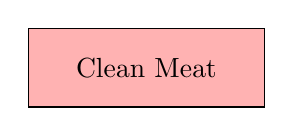
\begin{tikzpicture}[node distance=2cm]

\node (top1) [topic] {Clean Meat};
  
\end{tikzpicture}
\end{document}

